\documentclass[main.tex]{subfiles}
 
\begin{document}
 

\begin{lect}{2019-11-08}
    \section{ТФКП}\\
    Волковыский, Лунц, Араманович \q сборник задач по ТФКП

    \begin{Task}
        \[\sqrt[3]{i} \text{ - все значения}\]

        \begin{figure}[H]
            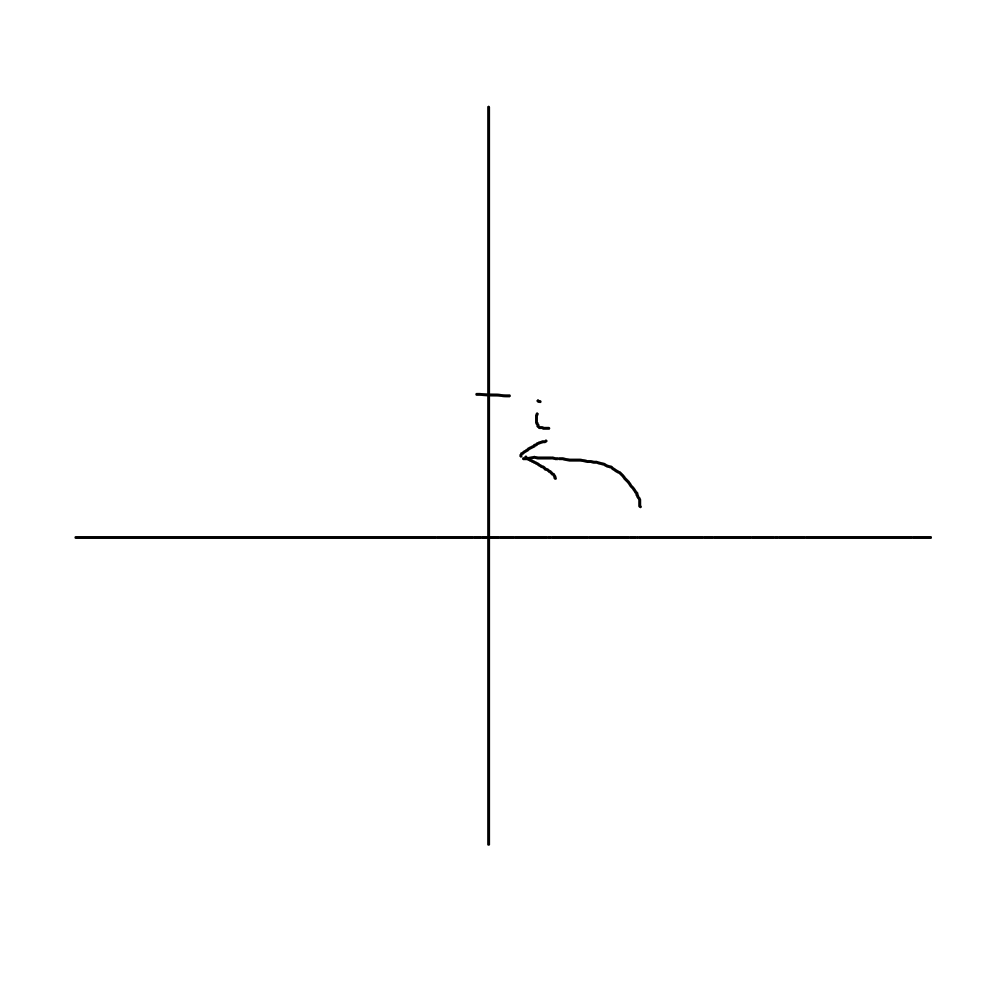
\includegraphics[width=7cm]{pics/13}
            \centering
        \end{figure}
        Так будем обозначать все аргументы (с большой буквы)
        \[\text{Arg } i = \frac{\pi}{2} + 2k\pi\]
        \[\sqrt[n]{z} = \sqrt[n]{\abs{z}} \left(\cos \frac{\text{Arg } z }{n} + 
        i\sin \frac{\text{Arg } z }{n}\right)\]
        \[\sqrt[3]{i} = \sqrt[3]{\abs{i}}(\cos \frac{\frac{\pi}{2} + 2\pi k}{3} + 
        i\frac{\sin \frac{\pi}{2} + 2\pi k}{3})\]
        \[ = 1(\cos(\frac{\pi}{6} + \frac{2\pi k}{3}) + i\sin(\frac{\pi}{6} + 
        \frac{2\pi k}{3}))\]
        \[z_1 = \frac{\sqrt{3}}{2} + \frac{i}{2}\]
        \[z_2 = -\frac{\sqrt{3}}{2} + \frac{i}{2}\]
        \[z_3 = -i \]
    \end{Task}

    \begin{Task}
        \[\sqrt{1 - i} \text{ - все значения}\]

        \[\real (1 - i) = 1\]
        \[\im (1 - i) = -1\]
        \[\abs{1 - i} = \sqrt{2}\]
        \[\text{Arg } (1 - i) = -\frac{\pi}{4} + 2\pi k\]
        \[\sqrt{1 - i} = \sqrt{\abs{1 - i}} (\cos \frac{\text{Arg } (1 - i)}{2} + 
        i\sin \frac{\text{Arg } (1 - i)}{2})\]
        \[k = 0 \q z_1 = \sqrt[4]{2} (\cos (-\frac{\pi}{8}) + i\sin( -\frac{\pi}{8}))\]
        \[\cos^2 \frac{\pi}{8} = \frac{1 + \frac{\sqrt{2}}{2} }{2}\]
        \[\sin^2 ( -\frac{\pi}{8}) = \frac{1 - \frac{\sqrt{2}}{2}}{2}\]
        \[\cos \left(- \frac{\pi}{8}\right) = \sqrt{\frac{1 + \frac{\sqrt{2}}{2}}{2}} = 
        \frac{\sqrt{2 + \sqrt{2}}}{2}\]
        \[\sin (-\frac{\sqrt{2 - \sqrt{2}}}{2})\]
        \[z_2 = -z_1 = -\sqrt[4]{2} \left(\frac{\sqrt{2 + \sqrt{2}}}{2} - 
        i\frac{\sqrt{2 - \sqrt{2}}}{2}\right)\]
    \end{Task}

    \begin{Definition}[Формула Эйлера]
        \[e^{ix} = \cos x + i\sin x \]
        \[e^{z_1 + z_2} = e^{z_1} \cdot e^{z_2}   \]
        \[e^{x + iy} = e^x (\cos y + i\sin y) \]
    \end{Definition}

    \begin{Definition}
        
        \[Ln z = w = u + iv  \ \rla \us{z \neq 0}{e\ ^w = z} \ \rla \ e^u
        (\cos v + i\sin v) =  z\]
        \[e^u = \abs{z}\]
        \[v = \text{Arg } z\]
        \[Ln z = \ln\abs{z} + i\text{Arg } z \qq\text{ комплексный лог.}\]
    \end{Definition}

    \begin{Definition}
        \[a > 0, \ b \in \R\]
        \[a^b = e^{b \ln a} \]
        По аналогии
        \[z_1 \neq 0 \q \Ra  z_1^{z_2} \os{def}{=} e^{z_2 \cdot Ln z_1}   \]
    \end{Definition}

    \begin{Utv}
        \[\text{Если } z_2 = n \in \N \text{ , то}\]
        \[z_1^n = \underbrace{z_1 \cdot z_1 ... z_1}_n \]
        \[\text{Если } z_2 = -n \text{, то}\]
        \[z_1^{-n} = \frac{1}{z_1 \cdot z_1 \cdot ... \cdot z_1} \]
        \[\text{Если } n = \frac{p}{q} \text{, то}\]
        \[z_1^n = (\sqrt[q]{z_1})^p\]
    \end{Utv}

    \begin{task}[1]
        Посчитать  $e^{\frac{\pi i}{4}}$
        \[e^{\frac{\pi i}{4}} = e^0 (\cos \frac{\pi}{4} + i\sin \frac{\pi}{4}) \]
        \[= \frac{\sqrt{2}}{2} + i\frac{\sqrt{2}}{2}\]
    \end{task}

    \begin{task}[2]
        Вычислить
        \[Ln(1  + i)\]

        \[\abs{1 + i} = \sqrt{2}\]
        \[\text{Arg } (1 + i) = \frac{\pi}{4} + 2\pi k\]
        \[\ln \sqrt{2}  + i(\frac{\pi}{4} + 2\pi k)\]
    \end{task}

    \begin{Task}[3]
        \[1 ^{\sqrt{2}}  \]
        \[1^{\sqrt{2}} = e^{\sqrt{2} Ln1} = e^{\sqrt{2}(i 2 \pi k)}  =  \]
        \[\abs{1} = 1\]
        \[\text{Arg } 1 = 0 + 2\pi k\]
        \[Ln 1 = i \cdot 2\pi k\]
        \[ = e^0(\cos 2\sqrt{2}\pi k + i\sin 2\sqrt{2}\pi k)\]
        \[ = \cos(2 \sqrt{2}\pi k + i\sin 2\sqrt{2}\pi k)\]
        \[k = 0 \q 1\]
        \[k = 1 \q \cos(2\sqrt{2}\pi) + i\sin(2\sqrt{2}\pi)\]
        Всюду плотно. Их бесконечно много и все на ед. окр.
    \end{Task}

    \begin{Task}[4]
        \[i^i - ?\]
        
         \[Ln i = \ln 1 + i(\frac{\pi}{2} + 2\pi k)\]
        \[i^i = e^{i \cdot Ln i} = e^{i \cdot i \cdot (\frac{\pi}{2} + 2\pi k)} = 
        e^{-(\frac{\pi}{2}  +2\pi k)} \]
        точки расположены на луче
    \end{Task}

    \begin{Task}[5]
        \[(1 + i)^{(1 - i)} \]

        \[e^{(1 - i) Ln (1 + i) } = \]
        \[Ln(1 + i) = \ln \sqrt{2} + i(\frac{\pi}{4} + 2\pi k)\]
        \[= e^{(1 - i)(\ln \sqrt{2} + i(\frac{\pi}{4} + 2\pi k))} \]
        \[= e^{\ln \sqrt{2} - (\frac{\pi}{4} + 2\pi k) + i(-\ln \sqrt{2} + \frac{\pi}{4} + 
        2\pi k)} \]
        \[= \sqrt{2} \cdot e^{- (\frac{\pi}{4} + 2\pi k)}( \cos (-\ln \sqrt{2} + 
        \frac{\pi}{4} + 2\pi k) + i\sin(-\ln \sqrt{2} + 
        \frac{\pi}{4} + 2\pi k)) \]
        \[= \sqrt{2} \cdot e^{- (\frac{\pi}{4} + 2\pi k)} (\cos (-\ln \sqrt{2} + \frac{\pi}{4}) 
        + i\sin(-\ln\sqrt{2} + \frac{\pi}{4})) \]
    \end{Task}

    \begin{Definition}
        \[\sin z = \frac{e^{iz} - e^{-iz}  }{2i}\]
        \[\cos z = \frac{e^{iz} + e^{-iz} }{2}\]
        \[\sh z = \frac{e^z - e^{-z} }{2}\]
        \[\ch z = \frac{e^z  + e^{-z} }{2}\]
        \[\ch z = \cos(iz) \qq \sh z = i \cdot \sin(iz)\]
        Отсюда получаются все тригонометрические тождества 
        \[\cos z = \ch(-iz) = \ch(iz)\]
        \[\sin z = \frac{1}{i}\sh(\frac{1}{i}z) = (-i) \cdot \sh(-iz) = i \cdot \sh(iz)\]
    \end{Definition}

    \begin{Task}[6]
        \[\text{Доказать} \sin(z_1 + z_2) = \sin z_1 \cos z_2 + \sin z_2 \cos z_1\]
        \[\sin z_1 \cdot \cos z_2 + \cos z_1 \cdot \sin z_2 = 
        \frac{e^{iz_1} - e^{-iz_1}  }{2i} \cdot \frac{e^{iz_2} + e^{-iz_1} }{2} +\]
        \[\frac{e^{iz_2} + e^{iz_2}  }{2} \cdot \frac{e^{iz_2} + e^{-iz_2}  }{2i} =  \]
        \[= \frac{e^{i(z_1  + z_2)} - e^{i(-z_1 + z_2)} +
        e^{i(z_1 - z_2)} - e^{-i(z_1 + z_2)}}  {4i}  + \] % косяк поправить
        \[+ \frac{e^{i(z_1 + z_2)} + e^{i(-z_1 + z_2)} - 
        e^{i(z_1 - z_2)} - e^{-i(z_1 + z_2)}}{4i} =\]
        \[= \frac{2e^{i(z_1 + z_2) - 2e^{-i(z_1 + z_2)} } }{4i} = \sin(z_1 + z_2)\]
    \end{Task}

    \begin{Task}[7]
        \[\sin(x + iy) \text{ через гипербол. ф.}\]

        \[\sin(x + iy) = \frac{e^{i(x + iy)} - e^{-i(x + iy)} }{2i} = 
        \frac{e^{ix} \cdot e^{-y} - e^{-ix} \cdot e^{y}   }{2i}\]
        Удобнее по-другому
        \[\sin(x + iy) = \sin(x)\cos(iy) + \sin(iy)\cos(x) = \sin x \cdot \ch y + 
        \cos x \cdot i\sh y = \]
        \[= \sin x \ch y + i \cos x \sh y\]
    \end{Task}

    \begin{Task}[8]
        \[w = \arcsin z \os{def}{\rla} \sin w = z\]
        \[\frac{e^{iw} - e^{iw}  }{2i} = z \]
        \[e^{-iw} = \frac{1}{e^{iw} } \]
        \[\frac{e^{iw} - \frac{1}{e^{iw} } }{2i} = z \]
        \[t = e^w \neq 0\]
        \[t - \frac{1}{t} = 2iz \ \rla \ t^2 - 1 = 2izt \]
        \[t^2 - 2iz - 1 = 0\]
        \[D = (-2iz)^2 + 4 = 4 - 4z^2\]
        \[t = \frac{2iz \pm \sqrt{4 - 4z^2}}{2} = iz \pm \sqrt{1 - z^2} \neq 0\]
        \[iw = Ln (iz \pm \sqrt{1 - z^2})\]
        \[w = \frac{Ln(iz \pm \sqrt{1 - z^2})}{i} = 
        -i Ln (iz \pm \sqrt{1 - z^2})\]
    \end{Task}

    \begin{Task}[9]
        \[\arcsin 2 = -i Ln(iz \pm \sqrt{1 - 4}) = -i Ln(2i \pm i\sqrt{3}) = 
        -i Ln(i(2 \pm \sqrt{3})) = \]
        \[Arg = \frac{\pi}{2} + 2\pi k\]
        \[\abs{ .. } = 2 \pm \sqrt{3}\]
        \[-i(\ln(2 + \sqrt{3}) + i(\frac{\pi}{2} + 2\pi k)) = -i\ln(2 + \sqrt{3}) + 
        \frac{\pi}{2} + 2\pi k\]
        \[= -i(\ln (2 - \sqrt{3}) + i(\frac{\pi}{2} + 2\pi k)) = -i\ln(2 - \sqrt{3}) + 
        \frac{\pi}{2} + 2\pi k\]
        \[2 - \sqrt{3} = \frac{1}{2 + \sqrt{3}}\]
        \[\ln(2  -\sqrt{3}) = -\ln(2 + \sqrt{3})\]
        \begin{figure}[H]
            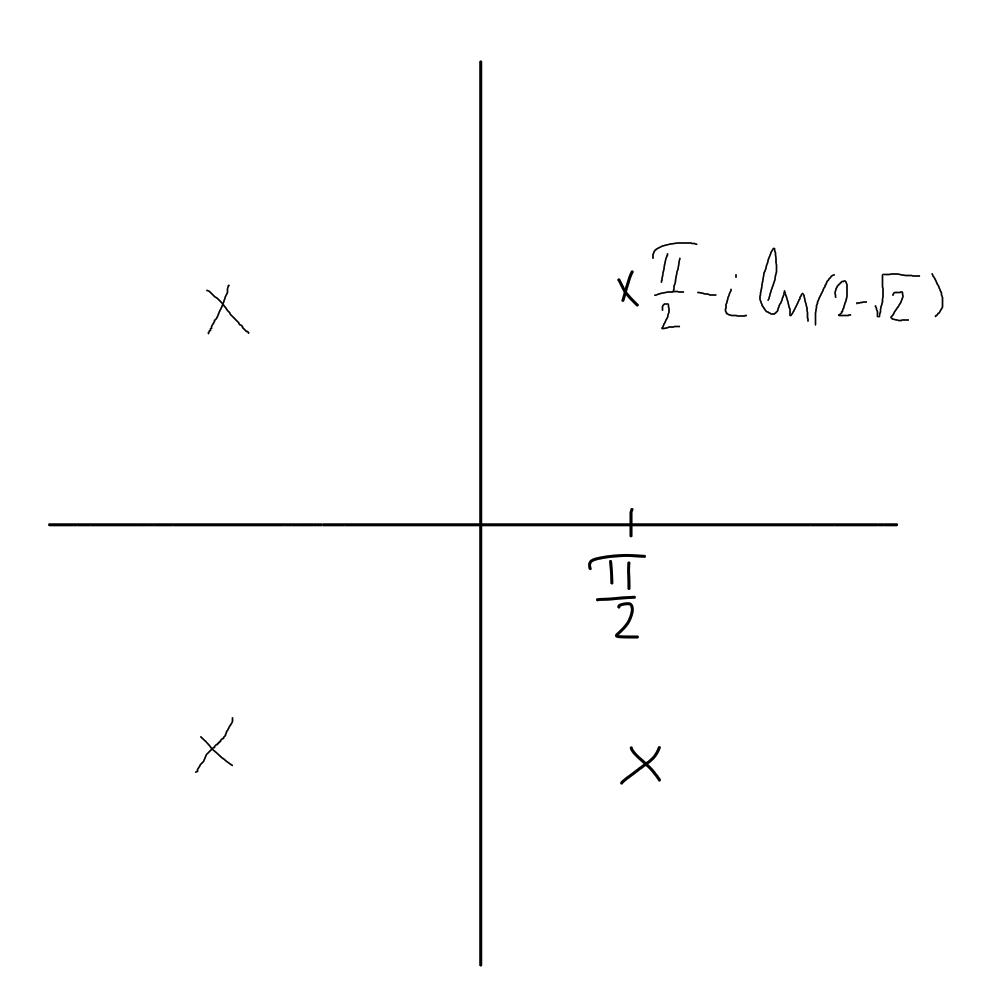
\includegraphics[width=5cm]{pics/14}
            \centering
        \end{figure}
    \end{Task}

    \begin{Task}[дз]
        \[\cos(x + iy) \qq \tg(x + iy) \qq (-2)^{\sqrt{2}} \qq (3 - 4i)^{1 + i}  \]
        \[\text{Найти } \arctg z \text{ через } Ln\]
        Надо сразу перейди к двойному арг.
        \[\tg w = \frac{\sin w}{\cos w} = \frac{e^{iw} - e^{iw}  }{i(e^{iw} + e^{iw}  )}\]
        \[\arctg (1 + 2i)\]
    \end{Task}
\end{lect}

\end{document}
